\documentclass[12pt, varwidth, border=5mm]{standalone}
\usepackage{tikz}
\usepackage{amsmath}
% Underlining package
\usepackage{ulem}
\usetikzlibrary{calc}
% \usepackage[a4paper, portrait, margin=1cm]{geometry}

\begin{document}
\section*{ }
    \begin{minipage}{0.55\textwidth}
  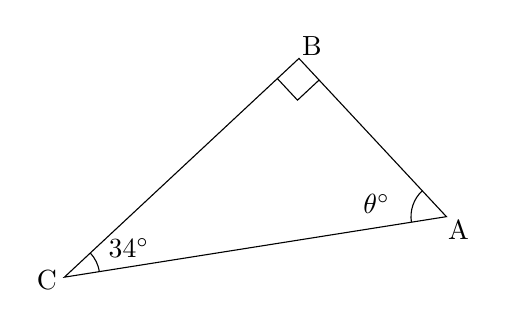
\begin{tikzpicture}[scale=1.5, baseline=(current bounding box.north)]

    \begin{scope}[rotate=9]
      \coordinate (A) at (0,0);
      \coordinate (B) at (3.274460368501429,0);
      \coordinate (C) at (intersection cs: first line={(A)--($(A)+(34:4cm)$)}, second line={(B)--($(B)+(180-56:4cm)$)});
      \draw (A) -- (B) -- (C) -- cycle;

      % Mark angles with arcs
      \draw ($(A)!0.3cm!(B)$) arc [start angle=0, end angle=34, radius=0.3cm];
      \draw ($(B)!0.3cm!(C)$) arc [start angle=180-56, end angle=180, radius=0.3cm];
      % \draw ($(C)!0.3cm!(A)$) arc [start angle=180+34, end angle=360-56, radius=0.3cm];
      % rt angle mark at C
      % \tkzMarkRightAng0le(A,C,B); % uses \usepackage{tkz-euclide}
      \draw ($(C)!0.25cm!(A)$) -- ($(C)!0.25cm!(A)!0.25cm!90:(A)$) -- ($(C)!0.25cm!(B)$);
      %  The ($(C)!0.3cm!(A)!0.3cm!90:(A)$) syntax is used to specify a point that is 0.3cm away from the point ($(C)!0.3cm!(A)$) in a direction that is perpendicular to the line connecting points C and A. This is achieved by first specifying the point ($(C)!0.3cm!(A)$) and then rotating it by 90 degrees around point A using the !angle:anchor syntax.

      % Label angles
      \node at ($(A)!-0.15cm!(B)$) {C};
      \node at ($(B)!-0.15cm!(C)$) {A};
      \node at ($(C)!-0.15cm!(A)$) {B};

      % Mark angles in degrees
      \coordinate (midBC) at ($(B)!0.5!(C)$);
      \node at ($(A)!0.60cm!(midBC)$) {$34^\circ$};

      \coordinate (midAC) at ($(A)!0.5!(C)$);
      \node at ($(B)!0.60cm!(midAC)$) {$\theta^\circ$};

      % \coordinate (midAB) at ($(A)!0.5!(B)$);
      % \node at ($(C)!0.55cm!(midAB)$) {<<angleCValueDisplay>>$^\circ$};

    \end{scope}
  \end{tikzpicture}
\end{minipage}%
\hfill
\begin{minipage}{0.4\textwidth}
  \begin{align*}
    \angle \text{A} &= 90^\circ - \angle \text{C} \\
    &= 90^\circ - 34^\circ  \\
    &= 56^\circ
  \end{align*}
\end{minipage}

\end{document}
